\chapter{the grand canonical ensemble}
\section{equilibrium between a system and a particle-energy reservoir} \label{4.1}
\begin{itemize}
	\item 系统 $A$ 和 particle-energy reservoir $A_\text{PER}$ 存在能量和粒子交换,
	\begin{equation}
		\begin{dcases}
			E_0 = E + E_\text{PER} \\
			N_0 = N + N_\text{PER}
		\end{dcases}, \quad \Omega_0(E_0, N_0) = \sum_{E, N} \Omega(E, N) \Omega_\text{PER}(E_0 - E, N_0 - N).
	\end{equation}
	
	\item 系统 $A$ 处于 $E, N$ 下的某一个 microstate 的概率为
	\begin{equation}
		P = \frac{\Omega_\text{PER}(E_0 - E, N_0 - N)}{\Omega_0} \simeq \frac{e^{- \beta (E - \mu N)}}{Z_\text{GC}}.
	\end{equation}
\end{itemize}

\section{a system in the grand canonical ensemble}
\begin{itemize}
	\item 考虑一个由 $\mathcal{N}$ 个全同子系统组成的系统, 总能量为 $\mathcal{E} = \mathcal{N} \braket{E}$, 总粒子数为 $N_\text{GCE} = \mathcal{N} \braket{N}$, 其中 $\braket{E} \equiv U, \braket{N}$ 分别是子系统能量和粒子数的期望值.
	
	\item $n_{i, N}$ 表示处于能级 $E_i$ 且有 $N$ 个粒子的子系统数量, 那么
	\begin{equation}
		\begin{dcases}
			\sum_{i, N} n_{i, N} = \mathcal{N} \\
			\sum_{i, N} n_{i, N} E_i = \mathcal{E} \\
			\sum_{i, N} n_{i, N} N = N_\text{GCE}
		\end{dcases}.
	\end{equation}
	
	\item $\{n_{i, N}\}$ 的微观态数量为
	\begin{equation}
		W\{n_{i, N}\} = \frac{\mathcal{N}!}{n_{0, 1}! \cdots n_{N_\text{EL}, N_\text{GCE}}!} \Longrightarrow \ln W\{n_{i, N}\} = \mathcal{N} \ln \mathcal{N} - \sum_{i, N} n_{i, N} \ln n_{i, N}.
	\end{equation}
	
	\item 最概然分布为
	\begin{equation}
		n_{i, N}^* = \mathcal{N} \frac{e^{- \beta (E_i - \mu N)}}{Z_\text{GC}} \approx \braket{n_{i, N}}.
	\end{equation}
	
	\item 并且有
	\begin{equation}
		\begin{dcases}
			\braket{N} = \frac{1}{\beta} \frac{\partial}{\partial \mu} \ln Z_\text{GC} \\
			\braket{E} = - \frac{\partial}{\partial \beta} \ln Z_\text{GC}
		\end{dcases}.
	\end{equation}
\end{itemize}

\section{the partition function and the grand potential}
\begin{itemize}
	\item 定义 fugacity,
	\begin{equation}
		z := e^{\beta \mu}.
	\end{equation}
	
	\item the partition function of the grand canonical ensemble 为
	\begin{equation}
		Z_\text{GC}(T, V, z) = \sum_{i, N} z^N e^{- \beta E_i} = \sum_{N = 1}^\infty z^N Z_\text{C}(E, V, N),
	\end{equation}
	and the grand potential is
	\begin{equation}
		\Phi_\text{G}(T, V, \mu) = - k_B T \ln Z_\text{GC}(T, V, z).
	\end{equation}
\end{itemize}

\section{particle number fluctuations in the grand canonical ensemble}
\begin{itemize}
	\item grand canonical ensemble 中的系统的粒子数和能量的方差是
	\begin{equation}
		\begin{dcases}
			\braket{(\Delta N)^2} = \braket{N^2} - \braket{N}^2 = \frac{1}{\beta^2} \frac{\partial^2}{\partial \mu^2} \ln Z_\text{GC} = \frac{1}{\beta} \Big( \frac{\partial N}{\partial \mu} \Big)_{T, V} \\
			\braket{(\Delta E)^2} = \frac{\partial^2}{\partial \beta^2} \ln Z_\text{GC} = - \Big( \frac{\partial U}{\partial \beta} \Big)_{V, z}
		\end{dcases},
	\end{equation}
	因此
	\begin{equation} \label{4.4.2}
		\begin{dcases}
			\frac{\sqrt{\braket{(\Delta N)^2}}}{\braket{N}} = \sqrt{\frac{k_B T}{V} \kappa_T} \\
			\braket{(\Delta E)^2} = \braket{(\Delta E)^2}_\text{C} + \bigg( \Big( \frac{\partial U}{\partial N} \Big)_{T, V} \bigg)^2 \braket{(\Delta N)^2}
		\end{dcases},
	\end{equation}
	通常 $\kappa_T \sim \frac{1}{P}$, 因此
	\begin{equation}
		\begin{dcases}
			\frac{\sqrt{\braket{(\Delta N)^2}}}{\braket{N}} \sim N^{- \frac{1}{2}} \\
			\frac{\sqrt{\braket{(\Delta E)^2}}}{U} \sim N^{- \frac{1}{2}}
		\end{dcases}.
	\end{equation}
	
	\begin{tcolorbox}[title=calculation:]
		考虑 $N(T, V, \mu)$, 注意对 homogeneous system $S dT = V dP - N d\mu$,
		\begin{equation}
			dN = \Big( \frac{\partial N}{\partial \mu} \Big)_{T, V} \underbrace{\Big( - \frac{S}{N} dT + \frac{V}{N} dP \Big)}_{= d\mu} + \Big( \frac{\partial N}{\partial T} \Big)_{V, \mu} dT + \Big( \frac{\partial N}{\partial V} \Big)_{T, \mu} dV,
		\end{equation}
		因此
		\begin{equation}
			\Big( \frac{\partial N}{\partial \mu} \Big)_{T, V} \frac{V}{N} = \Big( \frac{\partial N}{\partial P} \Big)_{T, V} = - \frac{\big( \frac{\partial V}{\partial P} \big)_{T, N}}{\big( \frac{\partial V}{\partial N} \big)_{T, P}},
		\end{equation}
		对 homogeneous system
		\begin{equation}
			\Big( \frac{\partial V}{\partial N} \Big)_{T, P} = \frac{V}{N},
		\end{equation}
		因此
		\begin{equation}
			\Big( \frac{\partial N}{\partial \mu} \Big)_{T, V} = - \frac{N^2}{V^2} \Big( \frac{\partial V}{\partial P} \Big)_{T, N} = \frac{N^2}{V} \kappa_T, \Longrightarrow \frac{\braket{(\Delta N)^2}}{N^2} = \frac{k_B T}{V} \kappa_T.
		\end{equation}
		
		\noindent\rule[0.5ex]{\linewidth}{0.5pt} % horizontal line
		
		代入 $z = e^{\beta \mu}$,
		\begin{equation}
			\braket{(\Delta E)^2} = - \Big( \frac{\partial U}{\partial \beta} \Big)_{V, z} = k_B T^2 \Big( \frac{\partial U}{\partial T} \Big)_{V, \mu} + k_B T \mu \Big( \frac{\partial U}{\partial \mu} \Big)_{T, V},
		\end{equation}
		且
		\begin{equation}
			\Big( \frac{\partial U}{\partial T} \Big)_{V, \mu} + \Big( \frac{\partial U}{\partial \mu} \Big)_{T, V} \Big( \frac{\partial \mu}{\partial T} \Big)_{V, N} = \Big( \frac{\partial U}{\partial T} \Big)_{V, N} = C_V,
		\end{equation}
		代入,
		\begin{equation}
			\braket{(\Delta E)^2} = k_B T^2 C_V + k_B T \Big( \mu - T \Big( \frac{\partial \mu}{\partial T} \Big)_{V, N} \Big) \Big( \frac{\partial U}{\partial \mu} \Big)_{T, V},
		\end{equation}
		注意 $\mu = \big( \frac{\partial F}{\partial N} \big)_{T, V}$, 因此
		\begin{align}
			\mu - T \Big( \frac{\partial \mu}{\partial T} \Big)_{V, N} &= \Big( \frac{\partial F}{\partial N} \Big)_{T, V} - T \frac{\partial}{\partial T} \Big|_{V, N} \Big( \frac{\partial F}{\partial N} \Big)_{T, V} \notag \\
			&= \Big( \frac{\partial F}{\partial N} \Big)_{T, V} - T \frac{\partial}{\partial N} \Big|_{T, V} \underbrace{\Big( \frac{\partial F}{\partial T} \Big)_{V, N}}_{= - S} \notag \\
			&= \Big( \frac{\partial (F + T S)}{\partial N} \Big)_{T, V} = \Big( \frac{\partial U}{\partial N} \Big)_{T, V},
		\end{align}
		所以
		\begin{equation}
			\braket{(\Delta E)^2} = \underbrace{k_B T^2 C_V}_{= \braket{(\Delta E)^2}_\text{C}} + k_B T \Big( \frac{\partial U}{\partial N} \Big)_{T, V} \Big( \frac{\partial U}{\partial \mu} \Big)_{T, V},
		\end{equation}
		最后注意到
		\begin{equation}
			\Big( \frac{\partial U}{\partial N} \Big)_{T, V} \Big( \frac{\partial N}{\partial \mu} \Big)_{T, V} = \Big( \frac{\partial U}{\partial \mu} \Big)_{T, V},
		\end{equation}
		得到
		\begin{equation}
			\braket{(\Delta E)^2} = \braket{(\Delta E)^2}_\text{C} + \bigg( \Big( \frac{\partial U}{\partial N} \Big)_{T, V} \bigg)^2 \braket{(\Delta N)^2}.
		\end{equation}
	\end{tcolorbox}
\end{itemize}

\section{examples}
\subsection{classical ideal gas}
\begin{itemize}
	\item 现在来考虑更一般的理想气体 (粒子可能有 internal degrees of motion), 此时
	\begin{equation}
		Z_\text{C}(T, V, N) = \frac{(Z_\text{C}(T, V, 1))^N}{N!},
	\end{equation}
	而
	\begin{equation}
		Z_\text{C}(T, V, 1) = V \phi(T).
	\end{equation}
	
	\item 理想气体的 $Z_\text{GC}$ 为
	\begin{equation}
		Z_\text{GC}(T, V, z) = \sum_{N = 1}^\infty z^N \frac{(V \phi(T))^N}{N!} = e^{z V \phi(T)},
	\end{equation}
	因此
	\begin{equation} \label{4.5.4}
		\begin{dcases}
			\Phi_G = - k_B T z V \phi(T) \\
			U = k_B T^2 z V \phi'(T) \\
			N = z V \phi(T) \\
			P = \frac{N k_B T}{V} \\
			S = N k_B \Big( - \ln z + z \frac{V}{N} (T \phi'(T) + \phi(T)) \Big)
		\end{dcases}.
	\end{equation}
\end{itemize}

\subsection{solid: a system of harmonic oscillators}
\begin{itemize}
	\item 固体的 Einstein model.
	
	\item 系统的 partition function 为 (固体每个粒子有 $D = 3$ 个振动方向, 对 $\phi(T)$ 作相应改动)
	\begin{equation}
		Z_\text{C}(T, V, N) = (Z_\text{C}(T, V, 1))^N, \quad Z_\text{C}(T, V, 1) = \phi(T) = \begin{dcases}
			\frac{1}{2 \sinh \frac{\hbar \omega}{2 k_B T}} & \text{quantum mechanically} \\
			\frac{k_B T}{\hbar \omega} & \text{classically}
		\end{dcases}.
	\end{equation}
	
	\item 系统 $Z_\text{GC}$ 为
	\begin{equation}
		Z_\text{GC} = \sum_{N = 1}^\infty z^N \phi^N(T) = \frac{1}{1 - z \phi(T)},
	\end{equation}
	因此
	\begin{equation} \label{4.5.7}
		\begin{dcases}
			N = \frac{z \phi(T)}{1 - z \phi(t)} \Longrightarrow z \phi(T) \simeq 1 - \frac{1}{N} \iff \beta \mu \simeq - \frac{1}{N} - \ln \phi(T) \\
			U = N k_B T^2 \frac{\phi'(T)}{\phi(T)} \\
			S = N k_B \Big( \ln \pi(T) + T \frac{\phi'(T)}{\phi(T)} + O({\textstyle \frac{\ln N}{N}}) \Big)
		\end{dcases}.
	\end{equation}
\end{itemize}

\subsection{solid-vapor equilibrium}
\begin{itemize}
	\item 考虑一个由固态和气态组成的系统, 具有温度 $T$ 和体积 $V$.
	
	\item 固态和液态具有相同的 fugacity, 结合 \eqref{4.5.4} 和 \eqref{4.5.7},
	\begin{equation}
		\frac{N_\text{g}}{V_\text{g} \phi_\text{g}(T)} = z_\text{g} = z_\text{s} \simeq \frac{1}{\phi_\text{s}(T)} \Longrightarrow \frac{N_\text{g}}{V_\text{g}} = \frac{P_\text{vapor}}{k_B T} = \frac{\phi_\text{g}(T)}{\phi_\text{s}(T)},
	\end{equation}
	代入单原子气体的 $\phi_\text{g}(T)$ 和 Einstein model 的 $\phi_\text{s}(T)$, 得到
	\begin{align}
		P_\text{vapor} &= k_B T \Big( \frac{2 \pi m k_B T}{h^2} \Big)^{\frac{3}{2}} \Big( 2 \sinh \frac{\hbar \omega}{2 k_B T} \Big)^3 e^{- \frac{\epsilon}{k_B T}} \notag \\
		&\overset{\text{classically}}{\simeq} k_B T \Big( \frac{m \omega^2}{2 \pi k_B T} \Big)^{\frac{3}{2}} e^{- \frac{\epsilon}{k_B T}},
	\end{align}
	其中 $\epsilon = \epsilon_\text{g} - \epsilon_\text{s}$ 是粒子处于固态和气态的能量差.
\end{itemize}

\section{thermodynamic phase diagram}
\begin{itemize}
	\item 一个典型的 $P$-$V$-$T$ phase diagram 如下 (来自 \href{https://en.wikipedia.org/wiki/File:PVT_3D_diagram-en.svg}{Wikipedia}):
	
	\begin{figure}[H]
		\centering
		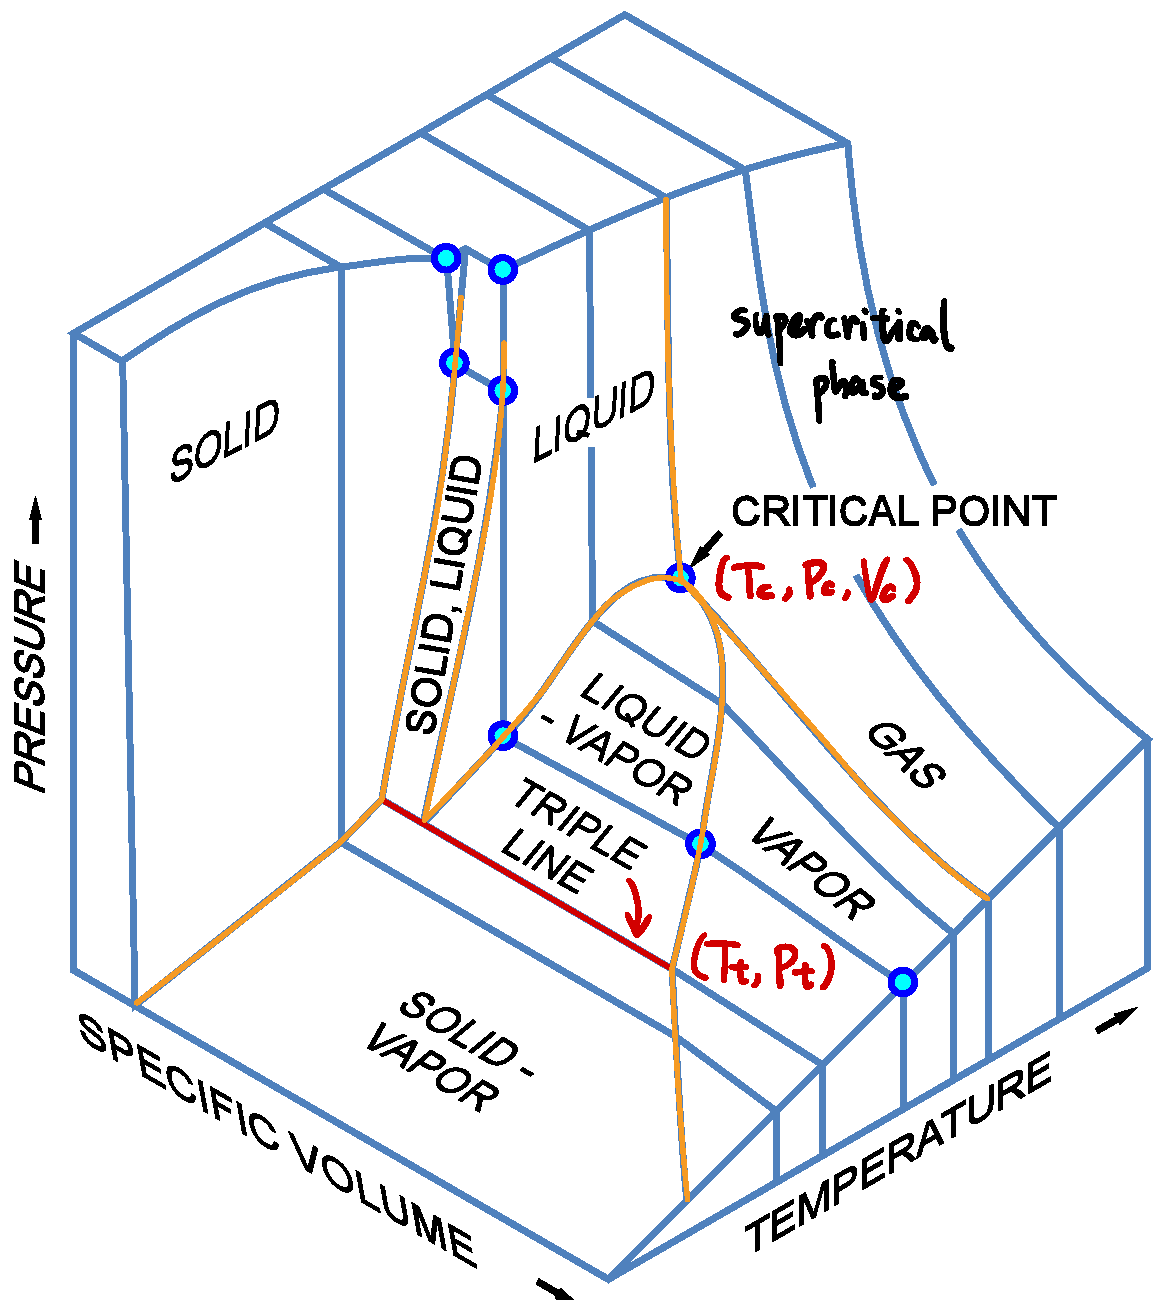
\includegraphics[scale=0.35]{figures/P-V-T phase diagram with comments.pdf}
		\caption{$P$-$V$-$T$ phase diagram}
	\end{figure}
	
	\item 几个重要的特征:
	\begin{itemize}
		\item triple line \& triple point.
		
		\item critical point.
		
		\item two-phase coexistence planes.
	\end{itemize}
\end{itemize}

\section{phase equilibrium and the Clausius-Clapeyron equation}
\begin{itemize}
	\item $P_\sigma(T)$ 描述 $P$-$T$ 面上的 phase boundary between two phases, 有 Clausius-Clapeyron equation,
	\begin{equation}
		\frac{dP_\sigma}{dT} = \frac{s_B - s_A}{v_B - v_A} = \frac{L}{T \Delta v},
	\end{equation}
	其中 $s$ 是 entropy per particle, $v$ 是 specific volume, $L$ 是 latent heat per particle (即 $A$ 相转化为 $B$ 相的吸热).
	
	\begin{tcolorbox}[title=proof:]
		两相共存要求 $\mu_A = \mu_B$, 对于 homogeneous systems,
		\begin{equation}
			s dT = v dP - d\mu \Longrightarrow d\mu = - s dT + v dP,
		\end{equation}
		因此
		\begin{equation}
			- s_A dT + v_A dP = - s_B dT + v_B dP \Longrightarrow \cdots
		\end{equation}
	\end{tcolorbox}
	
	\item 在 triple point, 3 条两相共存线的斜率保证任何一条共存线 (比如 $A$-$B$ 相共存线) 指向第三个相 ($C$ 相), 如下图所示.
	
	\begin{figure}[H]
		\centering
		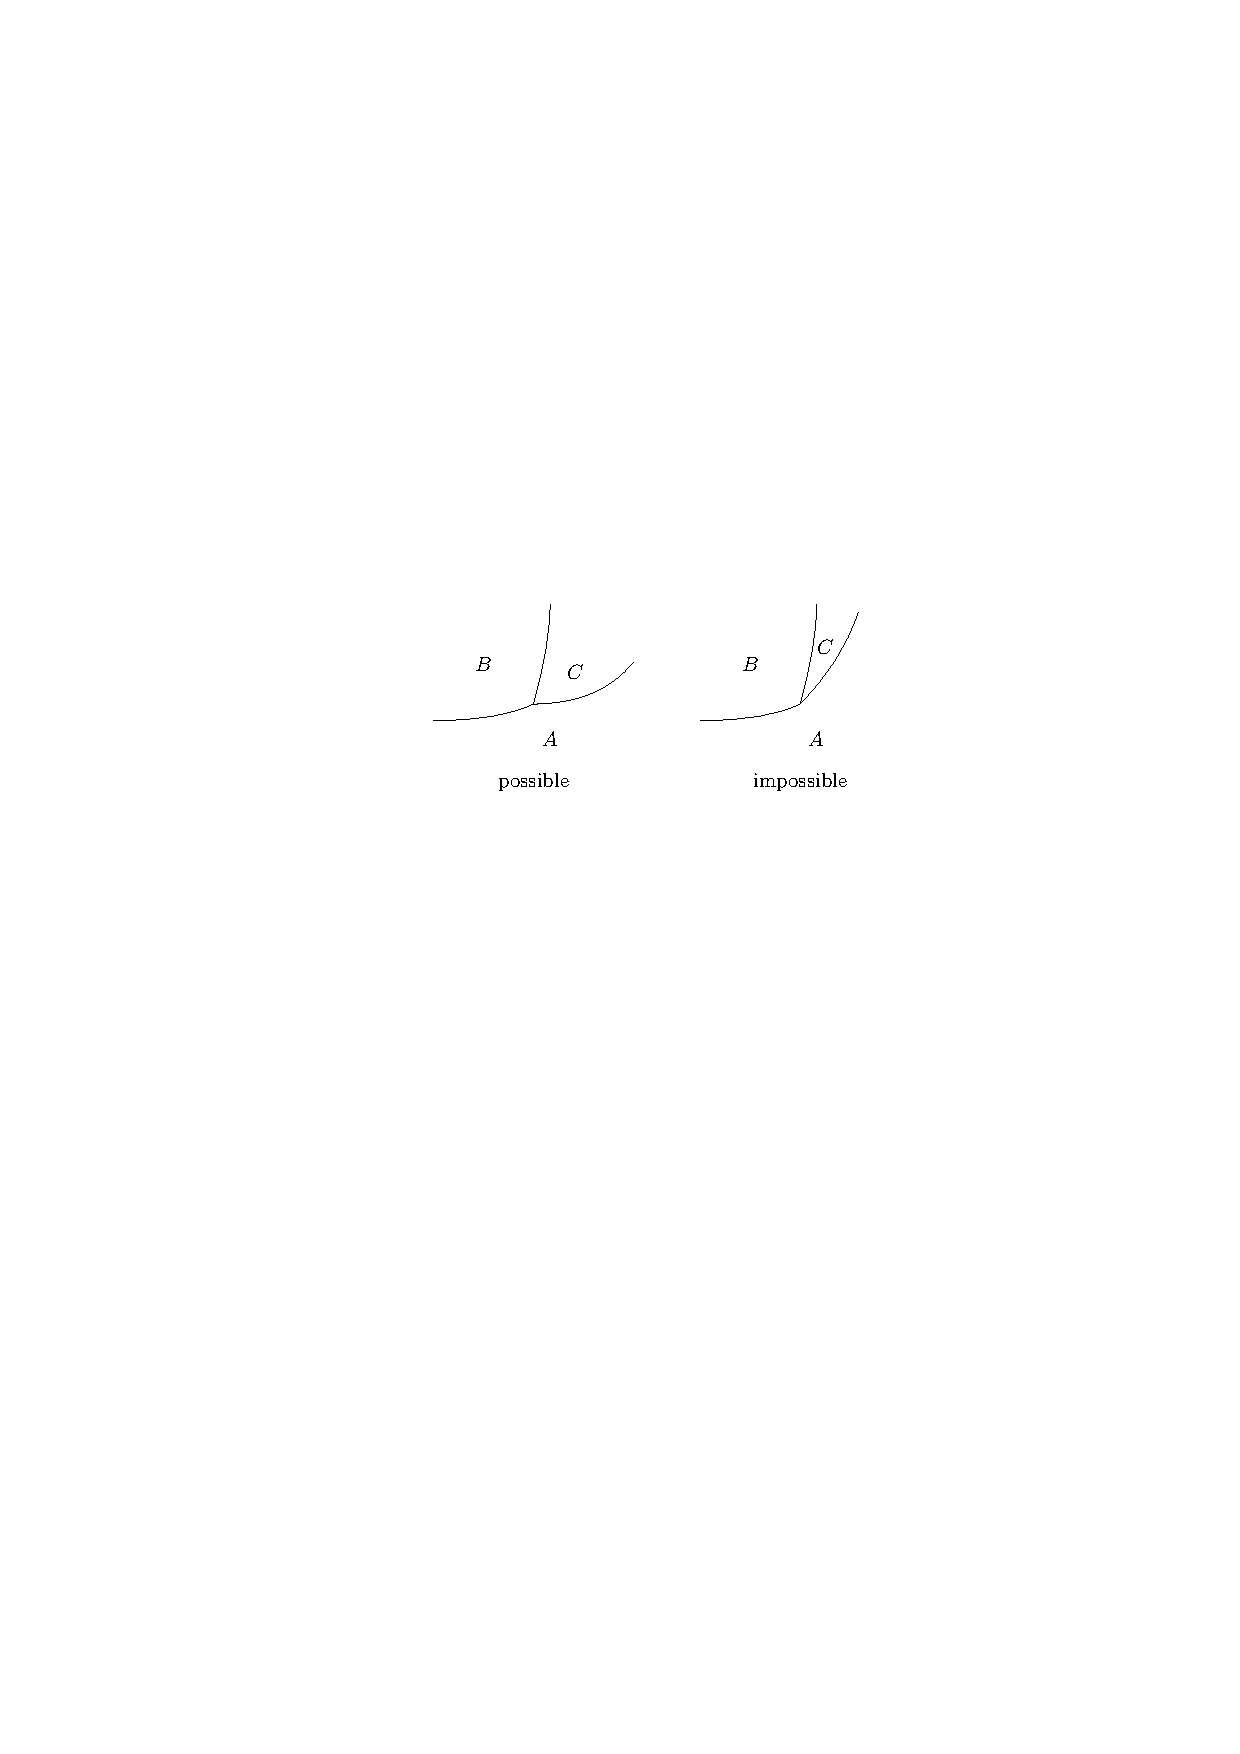
\includegraphics[scale=1]{figures/the slopes of 3 coexistence lines.pdf}
		\caption{the slopes of 3 coexistence lines.}
	\end{figure}
	
	\begin{tcolorbox}[title=proof:]
		注意到
		\begin{equation}
			\Delta s_{AB} + \Delta s_{BC} + \Delta s_{CA} \equiv 0, \quad \Delta v_{AB} + \Delta v_{BC} + \Delta v_{CA} \equiv 0,
		\end{equation}
		为了方便, 接下来分别用指标 $1, 2, 3$ 替代 $AB, BC, CA$.
		
		我们需要证明 $u_i = (\Delta v_i, \Delta s_i), i = 1, 2, 3$ 满足
		\begin{equation}
			\sum_{i = 1}^3 \alpha_i u_i = 0, \quad \text{with} \quad \alpha_i > 0,
		\end{equation}
		显然成立, $\alpha_i = 1$.
	\end{tcolorbox}
\end{itemize}
